\section{Design implementation using Lua scripting language}
After working on LibreCAD 3, I experimented with it by making some designs usign Lua scripting language which involes the concept of loops, conditional statements as well as functions.
\noindent In this project, I have made several lua scripts and run it on LibreCAD v3 to make various design. I have made design of water tank and various logos and some other impressive 2D design in LibreCAD using Lua scripting language. 
In LibreCAD v3, there is a dockable window for running lua scipts and the corresponding output is shown on the graphicscene which is main working window:
\begin{figure}[!ht]
\centering
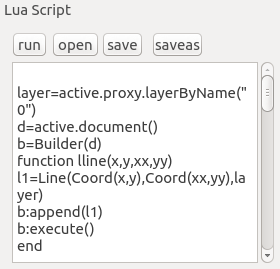
\includegraphics[scale=0.6]{images/lualogo/lua.png}                   
\caption{Lua Script DockWidget}
\end{figure}
\begin{figure}
\begin{center}
%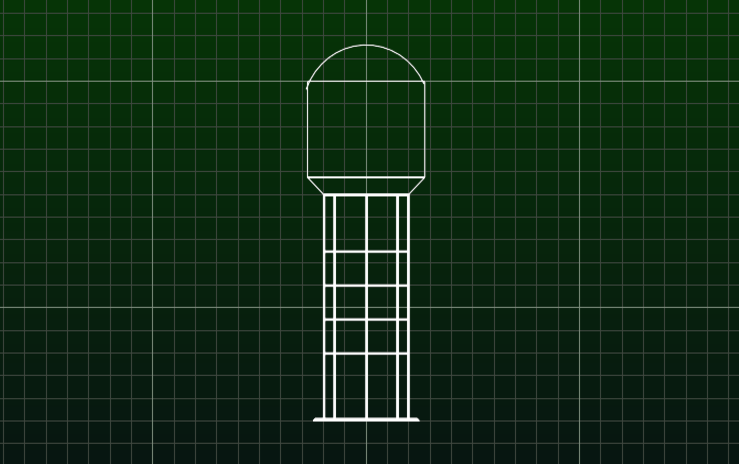
\includegraphics[scale=0.5]{images/lualogo/w2.png}
%\caption{Water Tank Model}
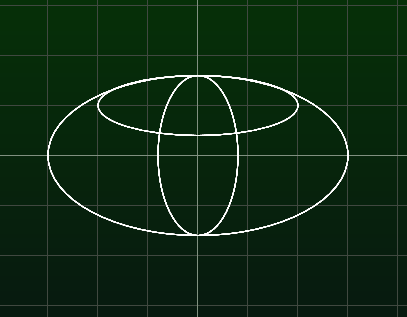
\includegraphics[scale=0.4]{images/lualogo/toyota.png}
\caption{Toyota Logo}

\includegraphics[scale=0.4]{images/lualogo/batman.png} 
\caption{Batman Logo}

\includegraphics[scale=0.3]{images/lualogo/chakra1.png}
\caption{Flower Design 1}
\end{center}
\end{figure}
